\chapter{\label{chap:chap3} Proposta de trabalho}


Podemos observar na topologia da Figura \ref{fig:fig1}, que os nodos não possuem um ponto centralizado de contato.
Em razão da topologia distribuida, se for necessário escalarmos a quantadidade de nodos na rede, a mesma não deverá sofrer impactos significativos de performance.
% Antes de sair falando sobre a figura seria interessante incluir um parágrafo introduzindo a proposta do trabalho.
% O que são os nodos? qual a ligação entre eles (relação) e qual a ligação entre os nodos e sensores? Podes falar um pouco da tecnologia de comunicação, da tecnologia empregada para construção dos nodos e sensores...


Nas seções a seguir abordaremos a arquitetura, módulos e submódulos que compõem o projeto.


\begin{figure}[htb!]
    \centering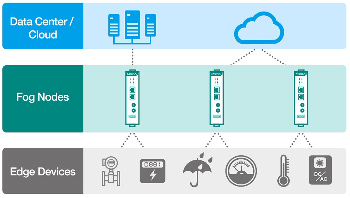
\includegraphics[width=.75\textwidth]{fig1.pdf}
    \caption%[This figure has a shorter caption now]%
    {\label{fig:fig1} Nodos da névoa.}
\end{figure}

\section{Arquitetura}

A fim de facilitar a compreensão da arquitetura deste projeto, a Figura \ref{fig:fig2} explicita a pilha de protocolos que o projeto fará uso para implementar as funcionalidades propostas.
% Arquitetura do que? denovo, deves explicar que tu irá definir uma pilha de protocolos que será utilizada juntamente com uma estrutura de organização arquitetural já previamente definida.

\begin{figure}[htb!]
    \centering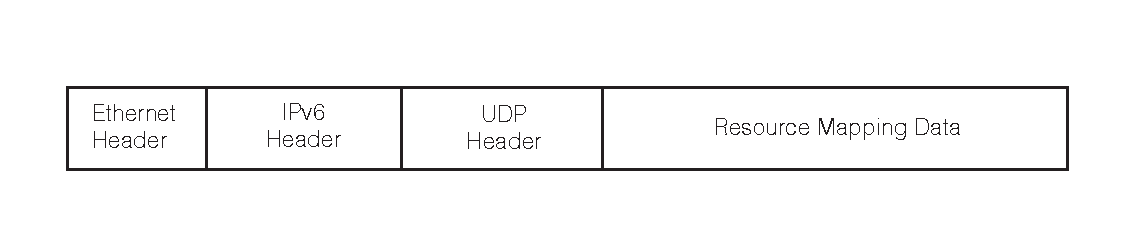
\includegraphics[width=.75\textwidth]{fig2.pdf}
    \caption%[This figure has a shorter caption now]%
    {\label{fig:fig2} Pilha de protocolos utilizada na implementação do projeto.}
\end{figure}

Dispondo do modelo de referência TCP/IP\cite{tanenbaum2011redes}, constituido de cinco camadas: física, enlace, rede, transporte e aplicação, este projeto utilizará IPv6 no nível de rede e UDP no nível de transporte.

A utilização de IPv6 na camada de rede justifica-se pela grande quantidade de endereços válidos na internet que o protocolo provê, pois após o firmamento da internet das coisas é possível que cada dispositivo tenha um endereço IP único.
Sendo assim, a escalabilidade, no que diz respeito a quantidade de endereços, está garantida.

Manter todos os nodos conectados, utilizando TCP por exemplo, despenderia uma quantidade de trafego significativo na rede. Além disso, o intuito desta implementação é transitar uma pequena quantidade de dados a cada requisição.
Portanto a utilização de datagramas UDP faz sentido neste projeto.
% Justificar o teu modelo proposto dizendo que manter o estado global de recursos acessível a todos os nodos é algo dificil e que um protocolo leve deve ser usado com o objetivo de permitir a escalabilidade com relação ao desempenho da solução.


\section{Módulos}

Nas próximas subseções esclareceremos as funcionalidades que o projeto deverá dispor.
Vale enfatizar que a descrição dos módulos apresentados referem-se a proposta de TCC I.
Consequentemente, o detalhamento de alguns módulos não serão abordados de forma aprofundada neste momento.


\subsection{Middleware}

O middleware utilizado neste trabalho realizará o mapeamento local nos nodos e descobrirá quais são os recursos disponíveis a serem compartilhados na névoa.
Utilizaremos uma simulação para realizar tal mapeamento local, portanto o mapeamento de fato não pertence ao escopo deste projeto.


%Apesar de não fazer parte do protocolo em sí, o middleware de mapeamento fornecerá interfaces de suma importância ao projeto.
%Este middleware implementará métodos de monitoramento e gerenciamento dos recursos.

%Abaixo elencaremos as principais funcionalidades que o middleware deverá implementar.
%\begin{itemize}
%   \item getLocalResources() - este método deverá retornar uma lista com id e nome dos recursos que estão interagindo com o nodo.
%  Também, deverá ser executado de forma continua pelo middleware, pois além de ser necessário que a lista de recursos locais sempre esteja atualizada é possível que um dos recursos pare de funcionar como o esperado.
%    \item getGlobalResources(ip) - este método utilizará o protocolo de mapeamento para obter a lista com id e nome dos recursos de um determinado IP.
%    \item getGlobalResourceValue(ip, resourceId) - este método utilizará o protocolo de mapeamento para obter o valor do recurso de um determinado IP.
%    \item setGlobalResource(ip, resourceId, newValue) - este método utilizará o protocolo de mapeamento para alterar o valor do recurso de um determinado IP.   
%\end{itemize}

\subsection{Descobrimento e sincronização}

Cada nodo da rede deve manter uma lista com os endereços IP`s que fazem parte do mapeamento. Juntamente à cada endereço IP, deverá haver uma lista com os recursos providos por ele.
Em vista disso, cada nodo da névoa possui um mapeamento global de recursos disponíveis na rede.

Quando um nodo entrar na rede pela primeira vez, deverá enviar um pacote para os endereços unicasts indicando os recursos que disponibilizará.
O Pseudocódigo \ref{alg:alg1} demonstra, de forma simplificada, a política de atualização que cada nodo deverá implementar.


\begin{algorithm}[htb]
    \begin{center}
        \begin{algorithmic}[1]
            \STATE \textbf{function} $\text{Police(ip, resources)}$
            \STATE \hspace{\algorithmicindent} \textbf{if} $\text{exists(ip)}$
            \STATE \hspace{\algorithmicindent} \hspace{\algorithmicindent} $\text{update(ip, resources)}$
            \STATE \hspace{\algorithmicindent} \textbf{else}
            \STATE \hspace{\algorithmicindent} \hspace{\algorithmicindent} $\text{insert(ip, resources)}$
        \end{algorithmic}
    \end{center}
    \caption[Política de atualização de recursos]%
        {\label{alg:alg1} Política de atualização de recursos.}%
    \end{algorithm}



A manutenibilidade da lista de recursos globais é relevante para que a implementação do protocolo tenha sucesso, pois a névoa deverá saber quando um nodo, ou recurso dele, deixou de fazer parte da rede.
Para tal, faz-se necessário a utilização de alguns mecanismos de controle.
Esses controles são realizados em duas esferas, uma trata do desvinculamento do nodo da rede e outra quando um recurso deixa de fazer parte dela.

O desvinculamento pode ser abordado de forma similar as mensagens de keep alive utilizadas no protocolo BGP, por exemplo.
Mensagens de keep alive são adotadas para que os nodos da rede avisem seus vizinhos que ainda estão operação, pois sem esse procedimento seria difícil
saber quando remover um IP da lista de recursos globais. Portanto, para manter a lista o mais atualizada possível, este protocolo implementará mensagens deste tipo.

No momento em que um nodo requisitar um recurso global da névoa, e este estiver fora de operação, o nodo que foi solicitado deverá enviar um novo pacote para os endereços unicasts indicando quais são os seus recursos existentes no momento.
O nodo solicitado percebe que este recurso não esta mais disponível porque recebeu na requisição o id do recurso, e este não está em sua lista local.
Lembrando que o nodo requisitado está consciente desta divergência em virtude da execução continua do método getLocalResources. Portanto, o gatilho para a atualização dos recursos na névoa
é disparado pelo primeiro nodo que requisitar um recurso inválido.


\section{Resultados esperados}

Espera-se que este trabalho resulte em um protocolo funcional a nível de prova de conceito e que seja capaz de descobrir, sincronizar e consumir recursos de dispositivos sob computação em névoa.
Além disso, temos como objetivo fazer com que a névoa configure-se de forma autônoma, ou seja, quando um recurso ou nodo entrar ou sair da rede, a mesma devará manter-se coerente.
% O que mais?

\section{Validação}

Para validarmos o funcionamento do protocolo, utilizaremos um simulador de dispositivos a ser definido no decorrer deste TCC.
Estes dispositivos executarão o middleware citado no item 3.2.1 deste trabalho.

\section{Cenários de teste}

\begin{itemize}
    \item Entrada de algum equipamento na rede e este anunciando seus recursos. 
    \item Atulização das listas globais quando algum equipamento deixar de responder as mensagens de keep alive.
    \item Utilização de recursos de nodos da rede.
    \item Desligamento de recursos de algum dispositivo da rede, e posterior a isso, a tentativa de acesso a esse recurso por algum nodo.
    O equipamento que perdeu o recurso deverá anunciar seus novos recursos atualizando a lista global dos outros nodos da névoa.
\end{itemize}









